% !TEX root = ../thesis-example.tex
%
\chapter{Hypothesis and objectives}
\label{sec:problematic}

\cleanchapterquote{Le fait de rêver est sans doute une des données, plus nombreuses qu'on ne le pense, qui, mieux encore que le soleil ou la pluie, placent les hommes de tout climat, de toute époque et de toute condition devant des problèmes identiques.}{Roger Caillois}{L'incertitude qui vient du rêve, 1956}

\section{The role of arousals on DRF variability}
\label{sec:problematic:arousals}

\section{Influence of sleep inertia on DRF}
\label{sec:problematic:inertia}

As \citet{conduit_poor_2004} rightly noticed, to reiterate an earlier quotation (section \ref{sec:dream-recall:theories:inertia}), \q{quite possibly, brain functioning underlying the reporting and non-reporting of dreams does not exist within the pre-sleeping period at all, but within the period just after awakening, when cognitive resources are in demand to recall and/or consolidate events which have just occurred within the previous sleeping period}. This is particularly interesting given that the \q{period just after awakening} is characterized by reduced vigilance, sleepiness and impaired performances, a state often referred to as sleep inertia. As \citet{trotti_waking_2016} clearly pointed out in the title of her article \q{waking up is the hardest thing I do all day}, sleep inertia is also usually experienced as unpleasant. Although its duration is not consensual and varies depending on the outcome measure used, it is generally admitted that most of the behavioral effects of sleep inertia dissipate progressively in the first 30 minutes post awakening. Severity of sleep inertia has been positively associated to several factors such as prior sleep deprivation, awakening near the circadian trough of body temperature, awakening in slow-wave sleep (see \citealp{tassi_sleep_2000} for a review) and some sleep disorders.

With regards to dream recall, the impaired cognitive functioning in the minutes following awakening could be indeed detrimental to recall and/or consolidation of dream memories \citep{conduit_poor_2004}. As pointed out by \citet{schredl_factors_2003}, it would be in consequence \q{promising to correlate inter-individual differences regarding the sleep inertia with DRF}. One could expect that low dream recallers would suffer from more acute sleep inertia detrimental effect and that this stronger impairment of cognitive functioning would in turn prevent a successful encoding of dream into long-term memory. By contrast, high dream recallers would suffer from less sleep inertia and would consequently have less difficulty encoding dreams into memory.

Very little attention has hitherto been devoted to this hypothesis, and no experimental studies have either supported or refuted it. In order to fill this gap, we designed a combined EEG-fMRI study to investigate the brain functional connectivity of high and low dream recallers in the minutes following awakening from a 45 minutes mid-afternoon nap (see Figure \ref{fig:intro:problematics-fmri-paradigm}) Resting-state scans were acquired before the nap, 5 min and 25 min after awakening to investigate the brain functional reorganization during sleep inertia in the two groups, and each scan was associated with a mental calculation task to measure the cognitive impairments of sleep inertia. We predicted that high dream recallers would show (1) more dream recall following awakening from sleep (2) a higher functional connectivity within the default mode network (see section \ref{sec:dream-research:attempts:dmn} and \ref{sec:dream-recall:param:neuro}) (3) less cognitive performance impairments, suggesting a faster recovery from sleep of regions involved in executive and memory processes. We hypothesized that the brain functional organization during sleep inertia would differ between high and low dream recallers and reflect behavioral differences in dream recall.

\begin{figure}[htb]
	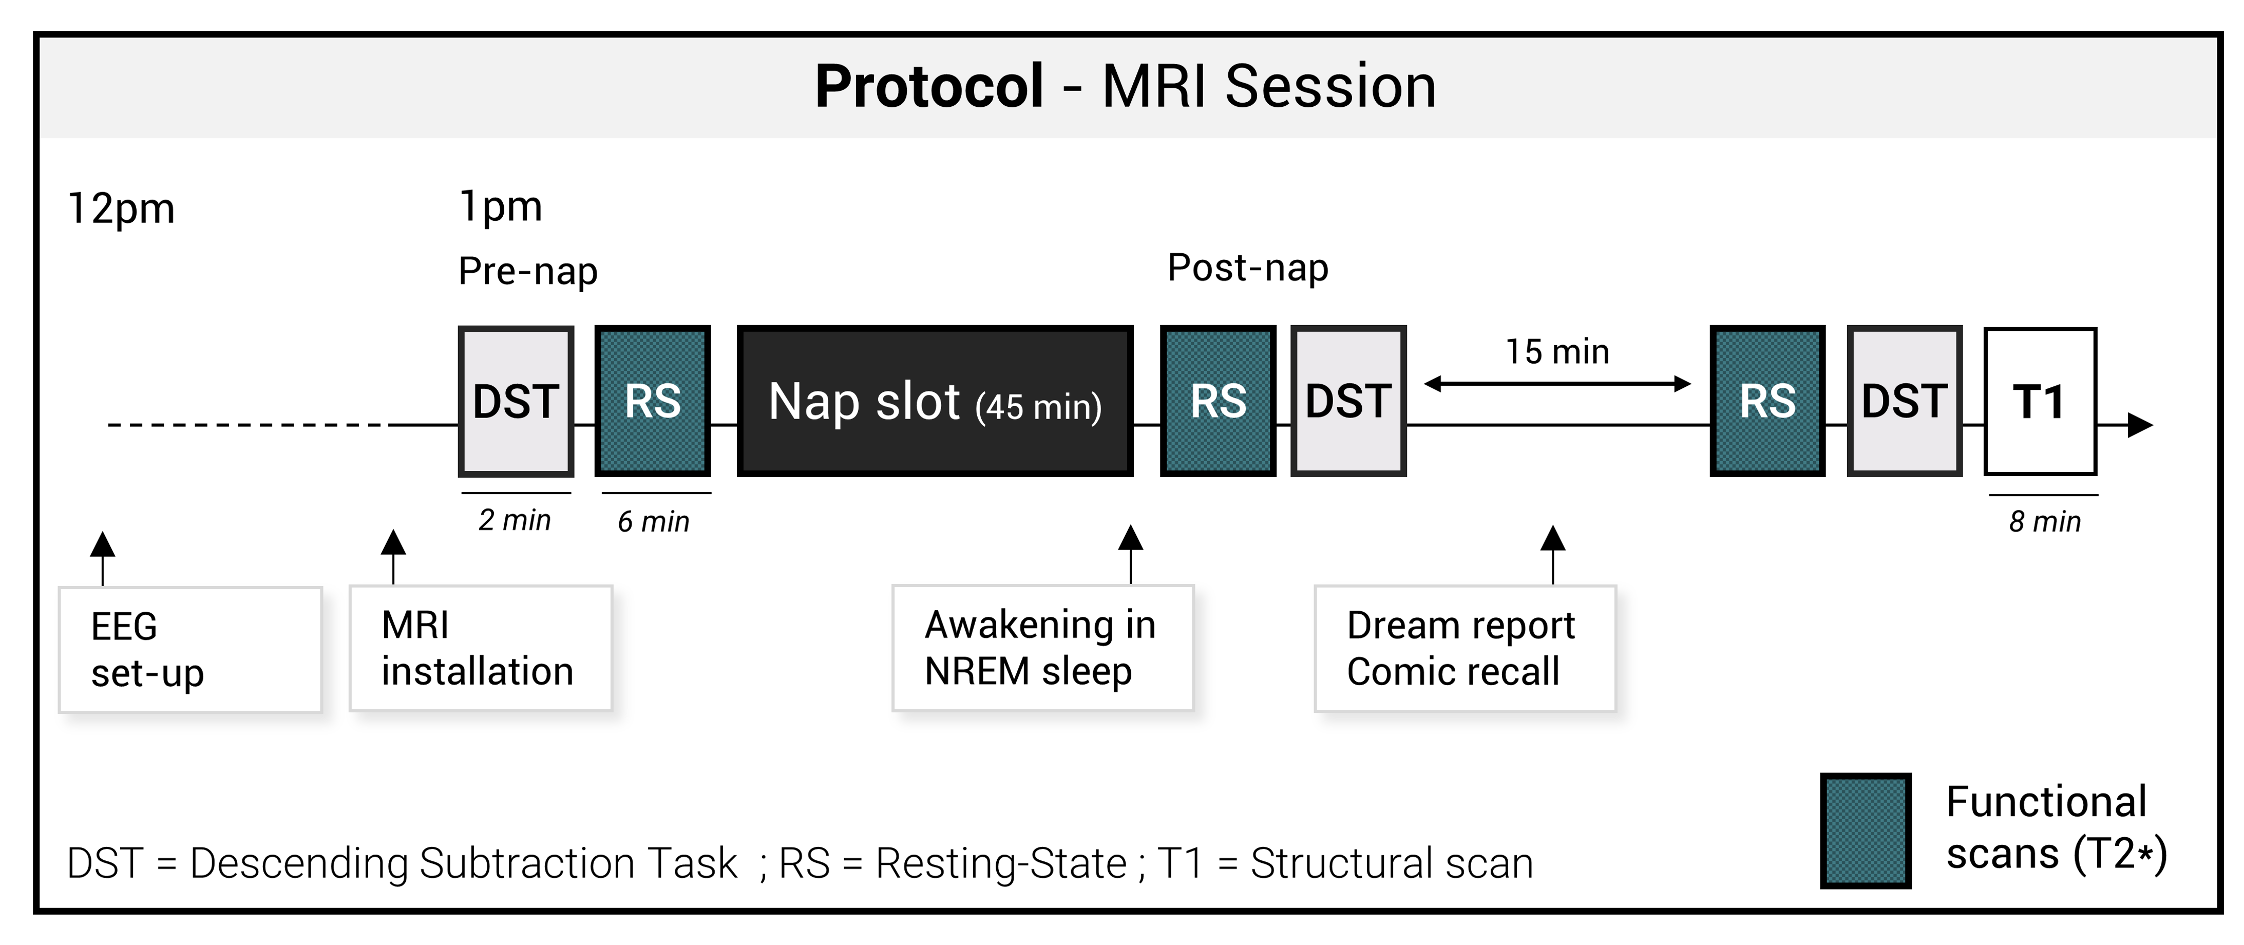
\includegraphics[width=\textwidth]{Fig/Intro/Intro_paradigm_fMRI/Intro_paradigm_fMRI.png}
	\caption[Experimental design of the fMRI study]{Experimental design of the sleep inertia fMRI study. After lunch at 11.30 am, participants were conducted to the neuroimaging center (CERMEP). During the first half hour, experimenters installed on the participant’s head a MRI compatible EEG cap. Participants were then installed in the MRI scanner. They read a 5 min cartoon during the calibration of the eye-tracking camera, and then performed a mental calculation  task (descending subtraction task, DST) for 2 minutes. The first resting-state scan was then acquired, with the instructions to remain awake and look at a central fixation cross on the screen. At the end of the scan, participants were informed that they could sleep during the next 45 min. At the end of the nap slot, participants were awakened, if they were sleeping, by calling their first name and the 2nd resting state scan was acquired. At the end of the scan, the 2nd DST was performed. During the following 10 minutes, subjects were asked about their dream(s) and sleep in the scanner and about the cartoon. Then the 3rd resting state scan and DST were performed (about 25 min after awakening). Finally, an 8-min T1 anatomical scan was acquired.Participants were selected if they reported and subsequently confirmed during a phone interview having a high or low DRF (DRF superior to 5 dream recalls per week and inferior to 2 dream recalls per month respectively) and having no sleep disturbances. Importantly, the night before the experiment, the subjects underwent a partial sleep deprivation (they were allowed to sleep between 5 am and 8 am) in order to facilitate sleep in the MRI scanner and heighten the sleep inertia effect.}
	\label{fig:intro:problematics-fmri-paradigm}
\end{figure}

\subsection{Sub-study 1: Brain networks dynamics during sleep inertia}
\label{sec:problematic:inertia:overview}

In addition with comparing the differential brain functional organization of high and low dream recallers during sleep inertia, this study offers the possibility to investigate thoroughly - by pooling the two groups - the brain networks changes across the sleep inertia period. Indeed, while the behavioral aspects of sleep inertia are well documented, only a limited amount of studies investigated its cerebral correlates until now. Using EEG, some studies have found a persistence of slow wave activity in the minutes following awakening, specifically in posterior areas, a phenomenon which has been suggested to represent the electro-physiological signature of sleep inertia \citep{ogilvie_falling_1992, ferrara_electroencephalographic_2006, marzano_recalling_2011, gorgoni_eeg_2015}. Using PET, \citet{balkin_process_2002} reported that the brain areas whose regional cerebral blood flow (rCBF) was increasing between 5 to 20 min post awakening were primarily anterior heteromodal areas (e.g. lateral prefrontal cortices, and anterior insula). They also reported shifts in the relative levels of rCBF between pairs of brain regions (orbitofrontal cortex and ventromedial caudate nucleus, dorsolateral prefrontal cortex and mesencephalic reticular formation) between 5 and 20 min post awakening, leading them to propose that recovery from sleep inertia could hinge on a resumption of normal levels of both rCBF and functional connectivity between brain areas. The latter hypothesis has been tested in two recent resting-state functional magnetic resonance imaging (fMRI) studies which investigated the variations in brain connectivity between pre-sleep wakefulness, nocturnal sleep (without previous sleep deprivation) and post-sleep
wakefulness \citep{wu_variations_2012, tsai_local_2014}. Using paired comparisons between pre- and post-sleep wakefulness, they found a decreased connectivity within the sensory-motor network at awakening but no alterations in the default mode network. This altered connectivity within the sensory-motor network is coherent with the poor motor performances observed at awakening but does not explain the impairments observed in other domains (e.g. cognitive tasks such as mental calculation, \citealp{tassi_sleep_2000, trotti_waking_2016}). Yet, some modifications of the default mode network connectivity could be expected at awakening since several neuroimaging studies showed consistent alterations of the default mode network connectivity during sleep, fatigue and/or falling asleep (see \citealp{picchioni_sleep_2013} for a review).

By looking at the brain and behavioral changes associated with sleep inertia, independently of the two group, our paradigm provides an ideal starting point to study, as wished by \citet{trotti_waking_2016} in her recent review, \q{the which and how functional brain networks are altered in the minutes following awakening}. Moreover, participants were partially sleep deprived on the night before and awakened from a 45 min mid-afternoon nap, in the deepest possible sleep stage (N3 sleep; see section \ref{sec:dream-research:sleep:stages}). Both sleep deprivation and awakening in N3 sleep have been associated with increased sleep inertia \citep{tassi_sleep_2000}. In addition with being ecological (short nights compensated by a daytime nap being common in young adults \citep{faraut_napping:_2016}, this paradigm allowed us to study sleep inertia in its most intensified form.

\subsection{Sub-study 2: Resting-state functional connectivity changes in high and low dream recallers}
\label{sec:problematic:inertia:resting-drf}

Another way to analyze the results of this study is to concatenate, for each subject, the three resting-state scans (i.e. pre-sleep, 5 min after awakening and 25 min after awakening). This approach allows to investigate the differences in functional connectivity at rest between high and low dream recallers.


\section{Sleep and dream habits in French students}
\label{sec:problematic:survey}

Epidemiological investigations in healthy subjects combining questions on both sleep and dreaming are relatively rare. Such measures are yet necessary to establish and keep up to date sleep and dream norms in the general population. Of particular interest is the college population, which is more at risk of suffering from sleep difficulties than the general population \citep{buboltz_sleep_2001, curcio_sleep_2006, forquer_sleep_2008, lund_sleep_2010}.

In order to recruit participants for our fMRI sleep study (section \ref{sec:problematic:inertia}), we have sent an announcement to several mailing lists of students from Lyon University. The announcement comprised a link to an online questionnaire about sleep and dream habits that participants had to fill out. The analysis of the responses provided up-to-date data on sleep and dream habits of a large sample of French college students, pertaining to different academic fields (i.e. humanities, science, medicine). Because our survey included relatively rare questions (e.g. frequency of recurrent and lucid dreams, sleepwalking, sleep-talking, sleep agitation), and thanks to a large sample of students including much more males than in previous studies (i.e. more than one third), we believe that this study will make a significant contribution to the limited number of previous epidemiological studies on sleep and dream habits of students.

\section{Contribution of day-residues and mundane waking-life events to dream content}
\label{sec:problematic:wle}

\section{An open-source software for sleep scoring and analysis}
\label{sec:problematic:software}

\subsection{Genesis and purpose}
\label{sec:problematic:software:genesis}

During my PhD thesis, I have been working extensively on polysomnographic sleep recordings, notably to score sleep microstructural events (e.g. arousals, rapid eye movements; see section \ref{sec:problematic:arousals}) and sleep stages (see section \ref{sec:problematic:inertia}). Traditionally, the scoring of sleep micro- and macro-structure is done visually and requires therefore a considerable investment of time and effort, in addition with being subject to both inter and intra-rater variability. Sleep scoring can also be done using automatic methods which have the advantage of being fast, reproducible and with generally good agreement with visual scoring \citep{berthomier_automatic_2007, lajnef_learning_2015}. Yet automatic scoring is far from being widespread and most sleep laboratories still rely on visual scoring, using either commercial softwares or in-house packages. In many cases, these softwares come with their own data and hypnogram file formats, and this heterogeneity can represent a substantial obstacle for sharing of algorithms and sleep data across laboratories or clinics. Some of the very few existing and up-to-date open sources alternatives allowing reading and scoring of sleep data are \fnurl{Phypno}{https://pypi.python.org/pypi/phypno} and \fnurl{SpiSOP}{http://www.spisop.org/}, yet they do not include graphical integration of automatic detection and are largely based on command-line options, which are hardly accessible for users with little or no programming knowledge.

It appears that there are currently no free, open-source and easy-to-use software capable of reading several file formats (both for data and hypnogram), and integrating automatic detection of sleep features within the graphical interface. Therefore, I developed during my PhD thesis an open-source software capable of filling this gap. At first intended for my personal use, it soon extended into a fully developed and comprehensive software, partly thanks to the help of my fellow PhD student \fnurl{Etienne Combrisson}{https://etiennecmb.github.io/}. This software was integrated into a broader neuroscientific suite named \fnurl{Visbrain}{http://visbrain.org/}, and the specific sleep module was named \textit{SLEEP}.

The primary aim of \textit{SLEEP} is to provide a fast and intuitive graphical user interface (GUI) to visualize and score polysomnographic sleep recordings. In order to be widely disseminated, the software must support a large range of data file formats, both proprietary (e.g. BrainVision) and public (e.g. European Data Format). It should also be able to handle the great heterogeneity in hypnogram formats (e.g. sampling frequency of the hypnogram, values assigned to each sleep stage). Finally, to provide a significant scoring aid, the software should include several automatic detection algorithms (e.g. spindles, K-complexes, slow-waves) and several signal processing tools (e.g. filtering, referencing). If these conditions are respected, we believe that this software could represent a major methodological development in the field of sleep research.

\section{Summary}
\label{sec:problematic:summary}

\begin{figure}[htb]
	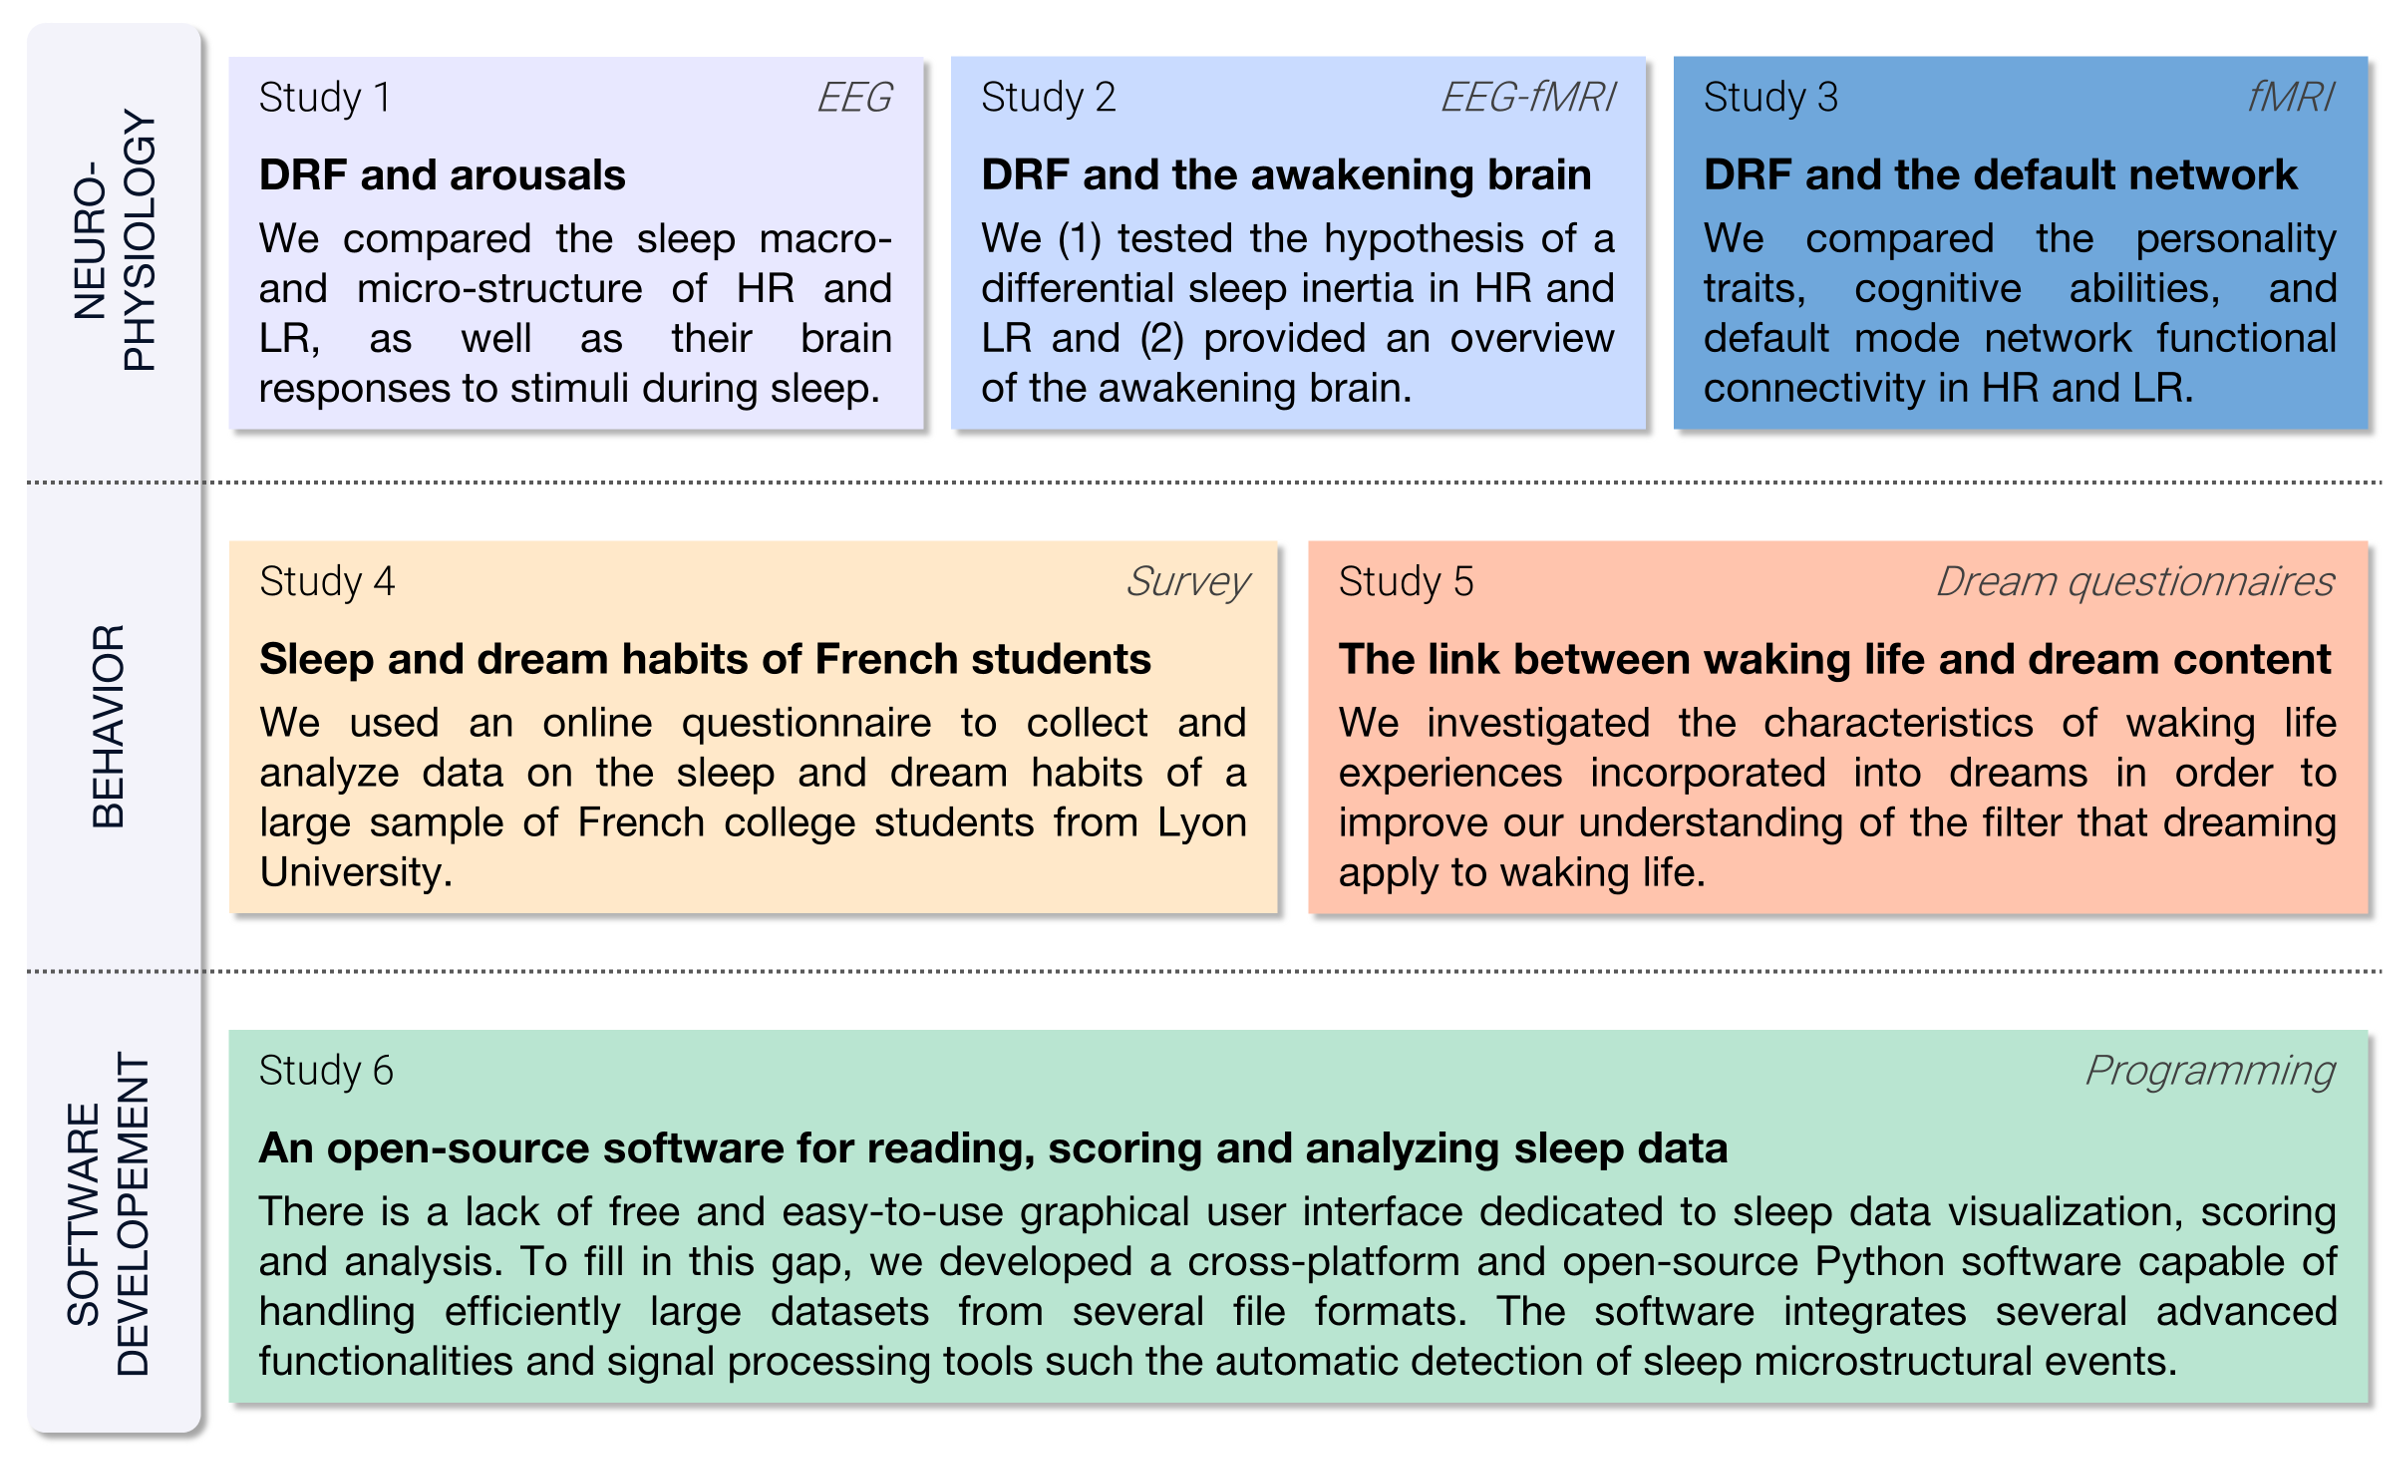
\includegraphics[width=\textwidth]{Fig/Intro/Intro_Problematics/Intro_Problematics.png}
	\caption[Summary of the studies conducted in this thesis]{Summary of the studies conducted in this thesis. In the first two studies, we investigated the neurophysiological correlates of dream recall frequency (DRF) with regards to nocturnal arousals and sleep inertia respectively. Studies 3 is an epidemiological survey of the sleep and dream habits in French college students from Lyon University. In study 4, we conducted a close analysis of the links between waking-life and dream content, with a special emphasis on the incorporation of remote and / or mundane memories. Finally, study 5 relates to the ongoing development of an open-source software to visualize, score and analyze polysomnographic sleep recordings.}
	\label{fig:intro:problematics-summary}
\end{figure}
